% ARTIGO BASE
% https://arxiv.org/pdf/2302.02162

\documentclass[conference]{IEEEtran}
\IEEEoverridecommandlockouts
% The preceding line is only needed to identify funding in the first footnote. If that is unneeded, please comment it out.
\usepackage{cite}
\usepackage{amsmath,amssymb,amsfonts}
\usepackage{algorithmic}
\usepackage{graphicx}
\usepackage{textcomp}
\usepackage{xcolor}
\usepackage{flushend}
\def\BibTeX{{\rm B\kern-.05em{\sc i\kern-.025em b}\kern-.08em
    T\kern-.1667em\lower.7ex\hbox{E}\kern-.125emX}}

\usepackage{caption}
\usepackage{subcaption}
\usepackage{tikz}
\usetikzlibrary{arrows.meta,positioning,calc}

\usepackage[ruled,vlined,linesnumbered]{algorithm2e}

% partes para adequar ao camera ready
\pdfminorversion=5 % força PDF 1.5
\pdfobjcompresslevel=0
\usepackage[left=1.62cm,right=1.62cm,top=1.9cm]{geometry}
% \usepackage[top=0.75in, bottom=0.75in, left=0.75in, right=0.75in]{geometry}

% original 0.90
\renewcommand{\baselinestretch}{1}
\setlength{\textfloatsep}{2.0pt plus 2.0pt minus 2.0pt}

\begin{document}


\title{Generic Title: Securing Semantic Communication}



\author{\IEEEauthorblockN{Prince~Nyarko\IEEEauthorrefmark{1},  Eirini~Eleni~Tsilopoulou\IEEEauthorrefmark{2},
André~Riker\IEEEauthorrefmark{1}\IEEEauthorrefmark{2}}
\IEEEauthorblockA{\IEEEauthorrefmark{1} Institute of Exact and Natural Sciences, Federal University of Par\'a, Brazil}
\IEEEauthorblockA{\IEEEauthorrefmark{2} Performance and Resource Optimization in Networks -- PROTON Lab\\ School of Electrical, Computer and Energy Engineering, Arizona State University, Tempe, AZ, USA}%%
}
%,castudillo@unicamp.br, weverton.cordeiro@inf.ufrgs.br, ariker@ufpa.br, gdecarvalho@brocku.ca
\maketitle

\begin{abstract}

Abstract ....

\end{abstract}

\begin{IEEEkeywords}
Federated Learning;
\end{IEEEkeywords}

\section{Introduction}
% INTRO
Modern Machine Learning

\section{Related Work}

Deep learning-based semantic communication has emerged as an alternative to conventional communication systems by prioritizing the preservation of meaning rather than exact bit-level reconstruction. Xie \textit{et al.} proposed DeepSC, an end-to-end Transformer-based framework that jointly learns semantic and channel representations for text transmission \cite{xie2021deepsc}. Beyond word-level reconstruction, Tang \textit{et al.} introduced a sentence-level semantic fidelity framework and a Semantic Similarity metric based on sentence embeddings, showing that BLEU alone may not adequately capture semantic equivalence between reconstructed and original sentences \cite{tang2023semanticfidelity}. This observation is particularly relevant to text semantic communication systems in which different surface forms may preserve the same underlying meaning.

Subsequent studies investigated semantic communication in multi-user and receiver-adaptation scenarios. Hu \textit{et al.} proposed MR\_DeepSC for one-to-many text semantic communication, where a shared Transformer-based transmitter serves multiple receivers and transfer learning is used to accelerate the training of additional receivers after freezing the transmitter parameters \cite{hu2022onetomany}. Liu \textit{et al.} further introduced knowledge distillation (KD) into Transformer-based text semantic communication for multiple users, demonstrating that teacher--student training can improve generalization and robustness under unseen interference while supporting model compression \cite{liu2024kdsemcom}. More recently, Nguyen \textit{et al.} proposed FRENCA, which trains a base-station encoder with a high-computing receiver, freezes the encoder, and adapts lower-computing receivers using transfer learning and KD \cite{nguyen2025optimizing}. Although these approaches establish the effectiveness of reusing a common semantic representation and adapting receiver models, their primary objectives are multi-user transmission, robustness, model compression, or heterogeneous computational capabilities rather than linguistic specialization.

Another research direction concerns cross-lingual and multilingual semantic communication. Xie \textit{et al.} investigated task-oriented semantic communication, including DeepSC-MT for machine translation \cite{xie2022task}. Cheng \textit{et al.} subsequently proposed a multilingual text semantic communication framework based on centralized and federated learning strategies \cite{cheng2025multilingual}. These studies demonstrate that semantic communication can operate across languages, but they rely on task-specific translation or multilingual training procedures. Efficiently extending an already trained text semantic communication model to an additional language while preserving most of its original parameters therefore remains a relevant problem.

Parameter-efficient fine-tuning offers a complementary approach to model adaptation. Hu \textit{et al.} introduced Low-Rank Adaptation (LoRA), which freezes pretrained weights and learns low-rank updates for selected Transformer layers, substantially reducing the number of trainable parameters compared with full fine-tuning \cite{hu2022lora}. Building on the above directions, this work investigates a shared-transmitter semantic communication architecture in which compact Student receivers are obtained through KD and subsequently personalized through LoRA. The shared semantic and channel encoders are retained across receivers, whereas each receiver can be specialized for a target language or application domain. Portuguese is used as the current experimental specialization.

\section{System Model and Proposed Method}

\subsection{Shared Transmitter and Personalized Receiver Architecture}

We consider a text semantic communication system with one shared transmitter and a set of personalized receivers. The communication architecture follows the DeepSC paradigm \cite{xie2021deepsc}. The shared transmitter contains the semantic encoder and channel encoder, while each receiver contains its own channel decoder, Transformer-based semantic decoder, and output prediction layer. Let the receiver set be
\begin{equation}
    \mathcal{R}
    =
    \left\{
        \mathcal{R}_1,
        \mathcal{R}_2,
        \ldots,
        \mathcal{R}_K
    \right\},
\end{equation}
where receiver $\mathcal{R}_k$ can be personalized for a particular target language or application domain. Examples include Portuguese, Spanish, French, or a domain-specific receiver. In the current experimental evaluation, Portuguese is considered as the target specialization, while the remaining cases represent the general architecture.

Let the source sentence be represented by
\begin{equation}
    \mathbf{s}=[w_1,w_2,\ldots,w_N],
\end{equation}
where $w_i$ denotes the $i$-th token of the input sentence. The shared semantic encoder $S_{\theta_s}(\cdot)$ maps the source sequence into a latent semantic representation
\begin{equation}
    \mathbf{h}=S_{\theta_s}(\mathbf{s}).
\end{equation}
The shared channel encoder $C_{\theta_c}(\cdot)$ subsequently transforms this representation into channel symbols,
\begin{equation}
    \mathbf{x}=C_{\theta_c}(\mathbf{h}).
\end{equation}
Before transmission, the channel symbols are power normalized. For receiver $k$, the received representation is written as
\begin{equation}
    \mathbf{y}_k
    =
    \mathcal{H}_k(\mathbf{x})
    +
    \mathbf{n}_k,
\end{equation}
where $\mathcal{H}_k(\cdot)$ denotes the channel transformation associated with receiver $k$ and $\mathbf{n}_k$ denotes channel noise. The implementation supports additive white Gaussian noise (AWGN), Rayleigh fading, and Rician fading channels.

At receiver $k$, the channel decoder reconstructs a semantic representation,
\begin{equation}
    \hat{\mathbf{h}}_k
    =
    C^{-1}_{\phi_{c,k}}(\mathbf{y}_k),
\end{equation}
which is processed by the personalized Transformer-based semantic decoder $S^{-1}_{\phi_{s,k}}(\cdot)$. Its output token distribution is
\begin{equation}
    \mathbf{p}_k
    =
    \mathrm{Softmax}\left(
    W_{o,k}
    S^{-1}_{\phi_{s,k}}(\hat{\mathbf{h}}_k)
    +
    b_{o,k}
    \right).
\end{equation}

The transmitter parameters $\theta_s$ and $\theta_c$ are shared and remain fixed during receiver personalization. Consequently, different receivers can reuse the same semantic representation while maintaining receiver-specific parameters for their language or domain specialization. Fig.~\ref{fig:personalized-receivers} illustrates this one-to-many architecture.

\begin{figure}[t]
    \centering
    \resizebox{\columnwidth}{!}{%
    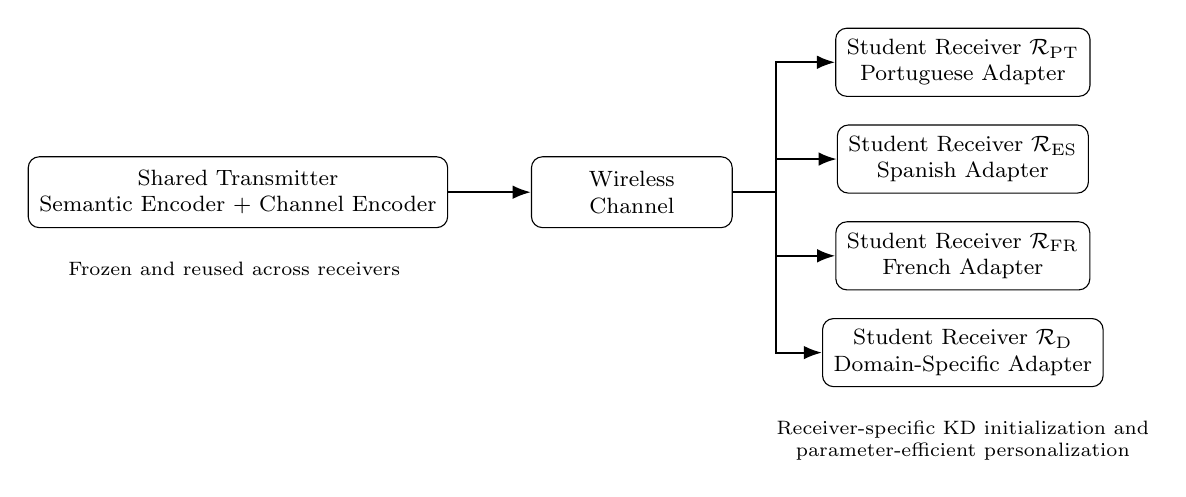
\begin{tikzpicture}[
        node distance=0.75cm and 1.05cm,
        >=Latex,
        every node/.style={font=\footnotesize},
        block/.style={
            draw,
            rounded corners,
            align=center,
            minimum width=2.55cm,
            minimum height=0.9cm,
            inner sep=4pt
        },
        receiver/.style={
            draw,
            rounded corners,
            align=center,
            minimum width=2.75cm,
            minimum height=0.82cm,
            inner sep=4pt
        },
        arrow/.style={->, thick}
    ]

    \node[block] (tx) {
        Shared Transmitter\\
        Semantic Encoder + Channel Encoder
    };

    \node[block, right=of tx] (channel) {
        Wireless\\Channel
    };

    \node[receiver, right=1.30cm of channel, yshift=1.65cm] (pt) {
        Student Receiver $\mathcal{R}_{\mathrm{PT}}$\\
        Portuguese Adapter
    };

    \node[receiver, below=0.35cm of pt] (es) {
        Student Receiver $\mathcal{R}_{\mathrm{ES}}$\\
        Spanish Adapter
    };

    \node[receiver, below=0.35cm of es] (fr) {
        Student Receiver $\mathcal{R}_{\mathrm{FR}}$\\
        French Adapter
    };

    \node[receiver, below=0.35cm of fr] (domain) {
        Student Receiver $\mathcal{R}_{\mathrm{D}}$\\
        Domain-Specific Adapter
    };

    \draw[arrow] (tx) -- (channel);

    \coordinate (split) at ($(channel.east)+(0.55,0)$);
    \draw[thick] (channel.east) -- (split);

    \draw[arrow] (split) |- (pt.west);
    \draw[arrow] (split) |- (es.west);
    \draw[arrow] (split) |- (fr.west);
    \draw[arrow] (split) |- (domain.west);

    \node[align=center, font=\scriptsize, below=0.30cm of tx] {
        Frozen and reused across receivers
    };

    \node[align=center, font=\scriptsize, below=0.30cm of domain] {
        Receiver-specific KD initialization and\\
        parameter-efficient personalization
    };

    \end{tikzpicture}%
    }
    \caption{Shared-transmitter architecture with multiple personalized Student receivers. The semantic and channel encoders are reused across receivers, while each receiver can be specialized for a target language or application domain. Portuguese is the language considered in the current experimental evaluation; the remaining receivers illustrate the general personalization architecture.}
    \label{fig:personalized-receivers}
\end{figure}


\subsection{Teacher--Student Receiver Distillation}

The adaptation procedure first constructs a compact Student receiver from a pretrained DeepSC model. The pretrained model is separated into a transmitter and a Teacher receiver. The transmitter contains the semantic encoder and channel encoder, whereas the Teacher receiver contains the channel decoder, Transformer semantic decoder, and output prediction layer. During Student training, both the transmitter and Teacher parameters remain frozen.

Given the same noisy channel representation $\mathbf{y}$, the Teacher and Student process the received semantic signal in parallel. The Student uses a reduced Transformer decoder compared with the Teacher and is optimized using the ground-truth sequence together with information distilled from the Teacher.

For a target sequence $\mathbf{t}$, the token reconstruction loss is defined using masked cross-entropy,
\begin{equation}
    \mathcal{L}_{\mathrm{CE}}
    =
    -\sum_{i\in\Omega}
    \log p_S(t_i\mid\mathbf{t}_{<i},\mathbf{y}),
\end{equation}
where $\Omega$ contains the non-padding token positions and $p_S(\cdot)$ denotes the Student output distribution.

Output-level knowledge is transferred from the Teacher through temperature-scaled Kullback--Leibler divergence,
\begin{equation}
    \mathcal{L}_{\mathrm{KD}}
    =
    T^2 D_{\mathrm{KL}}
    \left(
    p_T^{(T)}
    \parallel
    p_S^{(T)}
    \right),
\end{equation}
where $T$ is the distillation temperature and $p_T^{(T)}$ and $p_S^{(T)}$ denote the softened Teacher and Student output distributions, respectively.

Feature-level information is also transferred between the Transformer decoder representations. Let $\mathbf{f}_{T,i}$ and $\mathbf{f}_{S,i}$ denote the Teacher and Student decoder features at valid token position $i$. The implementation first normalizes the representations as
\begin{equation}
    \tilde{\mathbf{f}}_{j,i}
    =
    \frac{
        \mathbf{f}_{j,i}
    }{
        \lVert\mathbf{f}_{j,i}\rVert_2+\epsilon
    },
    \qquad j\in\{S,T\},
\end{equation}
and minimizes the mean-squared deviation of their cosine similarity from unity,
\begin{equation}
    \mathcal{L}_{\mathrm{feat}}
    =
    \frac{1}{|\Omega|}
    \sum_{i\in\Omega}
    \left(
        1-
        \tilde{\mathbf{f}}_{S,i}^{\mathrm{T}}
        \tilde{\mathbf{f}}_{T,i}
    \right)^2,
\end{equation}
where $\Omega$ contains the non-padding positions and $\epsilon$ is a small constant for numerical stability.

The overall Student training objective is
\begin{equation}
    \mathcal{L}_{\mathrm{Student}}
    =
    \lambda_{\mathrm{CE}}\mathcal{L}_{\mathrm{CE}}
    +
    \lambda_{\mathrm{KD}}\mathcal{L}_{\mathrm{KD}}
    +
    \lambda_{\mathrm{feat}}\mathcal{L}_{\mathrm{feat}}.
\end{equation}
In the current implementation, the loss weights are set to
$\lambda_{\mathrm{CE}}=0.6$,
$\lambda_{\mathrm{KD}}=0.3$, and
$\lambda_{\mathrm{feat}}=0.1$, with a distillation temperature of $T=2$.

This first stage produces a compact receiver that retains knowledge from the pretrained Teacher while allowing the transmitter to remain unchanged.

\subsection{LoRA-Based Receiver Personalization}

After knowledge distillation, each trained Student receiver can be used as the base model for receiver-specific personalization. Instead of fully fine-tuning receiver $\mathcal{R}_k$, Low-Rank Adaptation (LoRA) \cite{hu2022lora} is introduced into selected attention projections of its Transformer decoder. Each receiver maintains its own adaptation parameters while reusing the same frozen transmitter.

For a pretrained linear layer with weight matrix
$W_0\in\mathbb{R}^{d_{\mathrm{out}}\times d_{\mathrm{in}}}$,
LoRA keeps $W_0$ frozen and parameterizes its trainable update as
\begin{equation}
    \Delta W = BA,
\end{equation}
where
$A\in\mathbb{R}^{r\times d_{\mathrm{in}}}$ and
$B\in\mathbb{R}^{d_{\mathrm{out}}\times r}$.
The adapted transformation is therefore
\begin{equation}
    W =
    W_0 + \frac{\alpha}{r}BA,
\end{equation}
where $r$ is the LoRA rank and $\alpha$ controls the magnitude of the update.

For receiver $\mathcal{R}_k$, LoRA is applied to the query, key, value, and output projections of both the decoder self-attention and encoder--decoder attention modules. The original attention projection weights remain frozen, while receiver-specific low-rank matrices are optimized together with the output prediction head and LayerNorm parameters. The embedding layer remains frozen. Denoting the LoRA matrices of receiver $k$ by $A_k$ and $B_k$, the adapted transformation is
\begin{equation}
    W_k
    =
    W_0
    +
    \frac{\alpha_k}{r_k}
    B_k A_k.
\end{equation}

For a target sequence $\mathbf{t}_k$ associated with receiver $k$, the personalization objective is a masked token-level cross-entropy loss,
\begin{equation}
    \mathcal{L}_{\mathrm{adapt}}^{(k)}
    =
    \mathcal{L}_{\mathrm{CE}}
    \left(
        \mathbf{t}_k,
        \hat{\mathbf{t}}_k
    \right).
\end{equation}
Thus, different receivers can maintain distinct LoRA adapters for different languages or domains without modifying the common semantic transmitter.

In the current Portuguese specialization, an English source sentence is processed by the frozen shared transmitter and the Student receiver is trained against the Portuguese target sequence. Knowledge distillation is not repeated during this stage. Instead, the receiver first inherits the Teacher knowledge through the distillation stage and is subsequently personalized through parameter-efficient LoRA adaptation.

\section*{Acknowledgement}
This research was funded by CNPq (Brazil), under grants \#444978/2024-0, 201007/2025-8 and \#405026/2024-2.



\bibliographystyle{ieeetr}
\bibliography{paper,related_work}

\end{document}